\chapter{Capacitance}

\section{Introduction}

In this lab, we will explore th behavior of capacitors in circuits and how they interact with other circuit elements. Specifically, we will examin the behavior of current and voltage for charging and discharging  circuits, which comprise a resistor and a capacitor in series.

\section{Theory}

A capacitor is a device for storing electric charge and energy. For simplicity, an ideal capacitor can be considered as a pair of parallel conducting metal plates, as shown in Fig. \ref{fig:capacitor}. When a charge $+Q$ is placed on the upper plate and $-Q$ on the lower plate, a potential difference $V$ is established between the plates, and the quantities $Q$ and $V$ are related by the expression:
\begin{equation}
    Q = CV
\end{equation}
where the capacitance $C$ is determined by the size and separation of the plates.

\begin{figure}[h]
    \begin{center}
        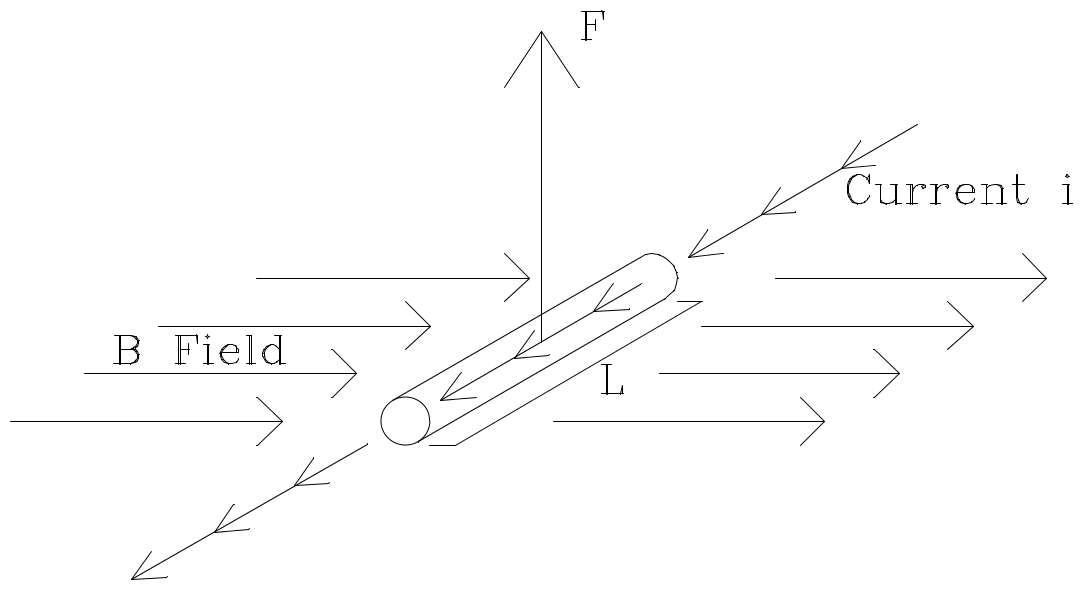
\includegraphics[width=0.5\textwidth]{./Exp4/pic/image1.png}
    \end{center}
    \caption{An Ideal Capacitor}
    \label{fig:capacitor}
\end{figure}

\subsection{Discharging a Capacitor}

If a wire is attached to the upper plate and then touched to the lower plate, charge will flow through the wire until the charge $q$ and potential difference $V$ are zero. (We will use $Q$ to indicate the initial charge and $q$ for the time dependent charge.) This process, known as discharging the capacitor, does not occur instantaneously. Instead, as the charge flows from one plate to the other, the potential difference decreases, and the current (or rate of change of charge) gradually diminishes. Since the rate of change is proportional to the amount of charge remaining, the current is initially large and then \emph{decays exponentially} with increasing time. Exponential growth or decay occurs whenever the rate of change of a quantity is proportional to the quantity present at that time. Exponentials are also characteristic of the growth rate of cells or organisms and the decay of radioactive isotopes.

The changing current which discharges a capacitor can be calculated as a function of time by considering the circuit shown in Fig.  \ref{fig:capcircuit1}. The capacitor $C$ is initially charged by a battery of emf $\varepsilon$, placing a charge $Q = C\varepsilon$ on the plates. When the switch is closed, a current $I$ flows in the circuit, and according to Ohm's Law the voltage drop across the resistance is $IR$.

\begin{figure}[h]
    \begin{center}
        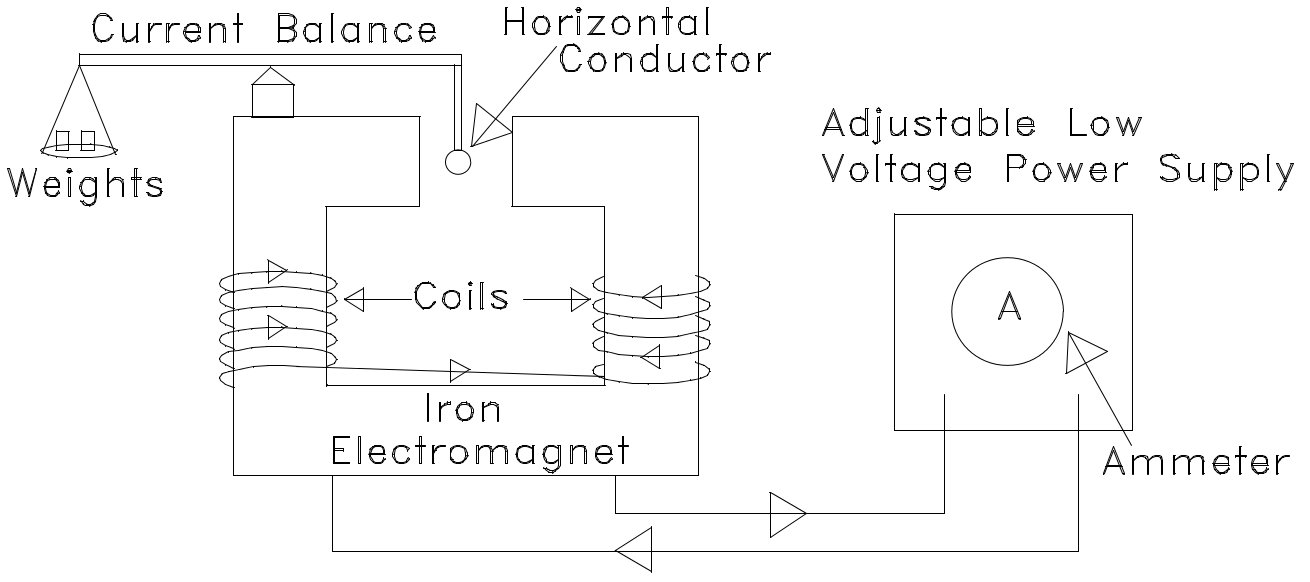
\includegraphics[width=0.4\textwidth]{./Exp4/pic/image2.png}
    \end{center}
    \caption{Discharging Circuit of a Capacitor}
    \label{fig:capcircuit1}
\end{figure}

The resistance may be a separate circuit element or merely the resistance of the wire itself. Since the sum of the voltage drops around the circuit must be zero, we obtain the equation:
\begin{equation}
    IR + \frac{Q}{C} = 0
\end{equation}

The equation can be rewritten in terms of charge alone from the definition of current, $\displaystyle I = dQ/dt \ \left(=\lim_{\Delta t\to 0} \frac{\Delta Q}{\Delta t}\right)$,
\begin{equation}
    R\frac{dQ}{dt} + \frac{Q}{C} = 0
    \label{eqn:diffcharge}
\end{equation}

Equation (\ref{eqn:diffcharge}) is a differential equation for $Q$ and has a solution which gives the time dependence of the charge
\begin{equation}
    Q(t) = C\varepsilon e^{-t/RC}
    \label{eqn:solcharge}
\end{equation}

Students familiar with calculus can verify this result by differentiating equation (\ref{eqn:solcharge}) and plugging back into equation (\ref{eqn:diffcharge}) to show that everything is satisfied. From the definition of current, $I = dQ/dt$, we find that
\begin{equation}
    I(t) = -\frac{\varepsilon}{R}e^{-t/RC}
    \label{eqn:dischargecurrent}
\end{equation}
Note that at $t=0$, when the switch is just closed, $I = -\varepsilon/R$. As time increases, the current $I(t)$ gets smaller and reaches zero as time goes to infinity.

\subsection{Charging a Capacitor}

The process of charging an uncharged capacitor has many similarities with the process of discharging discribed above. In this case, a battery with an emf of $\varepsilon$ volts is connected in series with a resistance $R$ and the capacitance $C$, as indicated in figure \ref{fig:chargecircuit}.

\begin{figure}[h]
    \begin{center}
        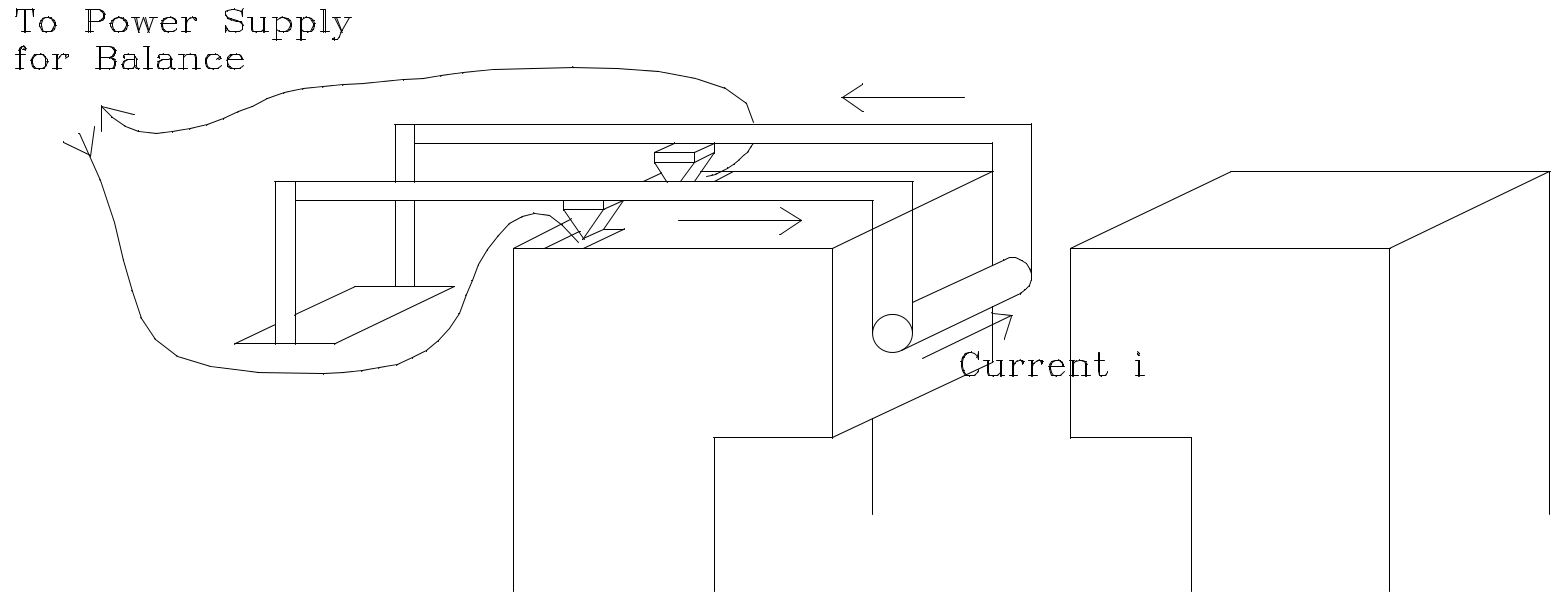
\includegraphics[width=0.4\textwidth]{./Exp4/pic/image3.png}
    \end{center}
    \caption{Charging Circuit of a Capacitor}
    \label{fig:chargecircuit}
\end{figure}

When the switch is first closed, there is no charge on the capacitor and thus no voltage across it, and the full voltage $\varepsilon$ appears across $R$, causing maximum current $I$ to flow. As the capacitor becomes charged, the voltage-drop $IR$ (and thus the current $I$) gradually decreases. $I$ approaches zero as the capacitor is charged toward its maximum potential difference of $\varepsilon = Q/C$. \myskip

The equation which indicates the sum of voltage drops around the circuit loop at any time during the charging is:
\begin{equation}
    \varepsilon = IR + \frac{Q}{C}
\end{equation}
Again, this can be converted to a \emph{differential equation}, the solution of which is:
\begin{equation}
    I(t) = \frac{\varepsilon}{R}e^{-t/RC}
    \label{eqn:chargecurrent}
\end{equation}

Comparing equation (\ref{eqn:dischargecurrent}) with (\ref{eqn:chargecurrent}), we note that the current for discharging a capacitor from a given potential $\varepsilon$ decreases in time identically to the current for charging the capacitor through the same resistance to the same final voltage $\varepsilon$. The difference in the sign of $I$ indicates, of course, that the two currents flow in opposite directions.

\subsection{Graphical Presentation of Exponential Decay}

In equations (\ref{eqn:dischargecurrent}) and (\ref{eqn:chargecurrent}), the symbol $e$ stands for the constant $2.71828\cdots$, the \emph{base of natural logarithms}. A graph of the function $y = ae^{-x/b}$ is given in figure \ref{fig:expgraph}, where $y=a$ at $x=0$ and then decays exponentially as $x$ increases, reaching a value of $y = ae^{-1} = 0.37a$ at $x=b$.

\begin{figure}[h]
    \begin{center}
        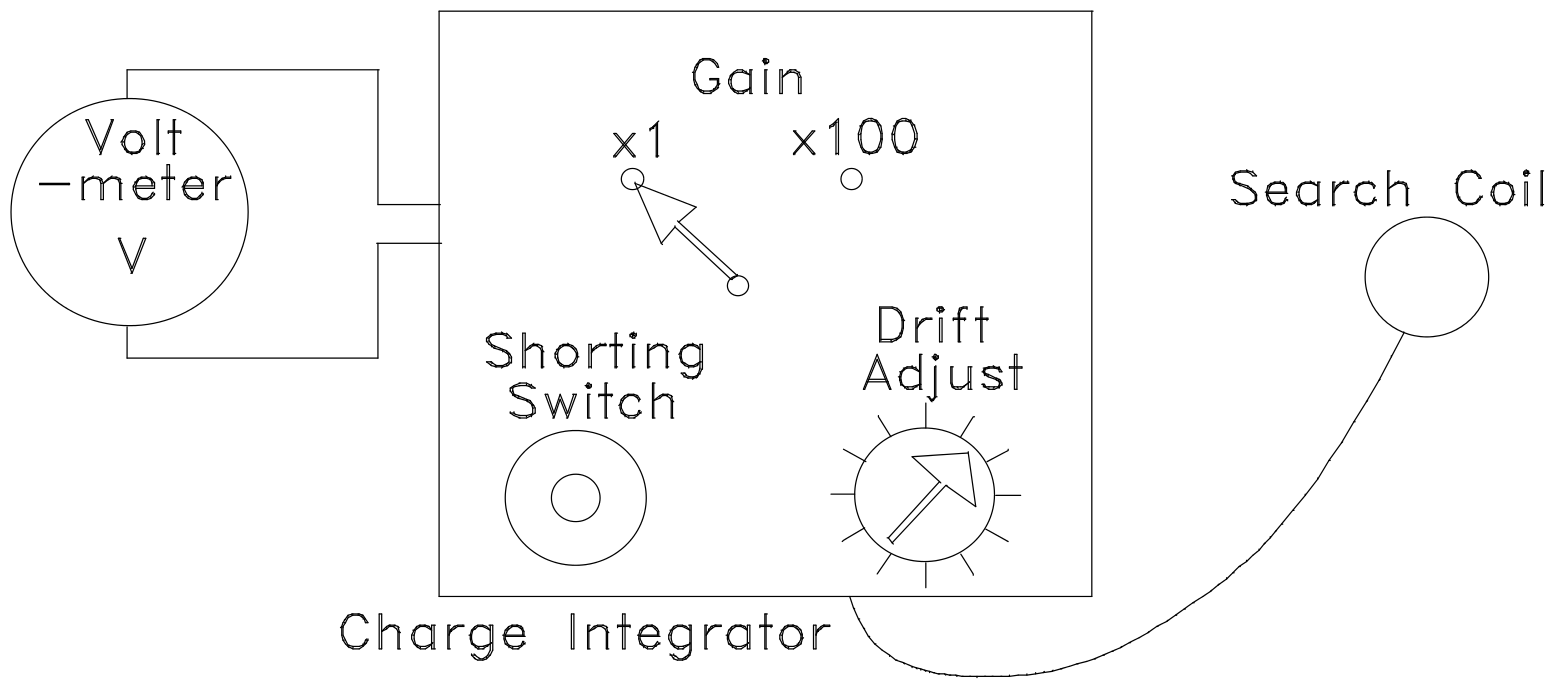
\includegraphics[width=0.9\textwidth]{./Exp4/pic/image4.png}
    \end{center}
    \caption{Graph of $y=ae^{-x/b}$}
    \label{fig:expgraph}
\end{figure}

Although it is possible to determine the values of $a$ and $b$ from experimental results plotted on such a curve, it is more informative to plot $\ln\,y$ versus $x$. Taking the natural logarithm (\ln) of $y=ae^{-x/b}$ yields:
\begin{equation}
    \ln\,y = \ln\,a + \ln\,e^{-x/b} = \ln\,a - \frac{x}{b}
    \label{eqn:logslope}
\end{equation}
which is a linear equation in $x$ representing a straight line with slope $-1/b$, if $\ln\,y$ is plotted against $x$ as in figure \ref{fig:logplot}. Linear equations are much easier to deal with. \myskip

\begin{figure}[h]
    \begin{center}
        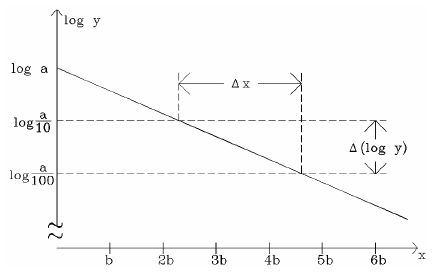
\includegraphics[width=0.8\textwidth]{./Exp4/pic/image5.png}
    \end{center}
    \caption{Plot of $\log\,y$ versus $x$}
    \label{fig:logplot}
\end{figure}

In the present experiment, $y$ repensents the current $I$; $x$ is the time $t$; $a$ is the initial value of $I$; and $b$ is the time constant $RC$. \myskip

\section{Procedure}

\subsection{Large RC-charging}

Fig. \ref{fig:largerccharge} shows the circuit to be wired for measuring the current $I$ as a function of time for charging a capacitor $C$ through a resistance $R$ to a voltage $\varepsilon$. For this part of the lab you will use the bank of three large capacitors which are attached to a piece of wood with three switches and the label ``$30\,\mathrm{MFd}$''. (In this case the prefix ``M'' in MFd indicates micro, $\mu$, or $10^{-6}$.) Be sure to use a low-voltage (15 volts max.) power supply and to connect the positive terminal on the power supply to the positive terminal on the microammeter. Before closing the switch to the power supply and starting each new measurement, momentarily connect a low resistance across the capacitor in order to start with no charge on the capacitor plates. It is important to note that the resistance $R$ being used for your measurements is the internal resistance of the ammeter\myskip
\begin{figure}[h]
    \begin{center}
        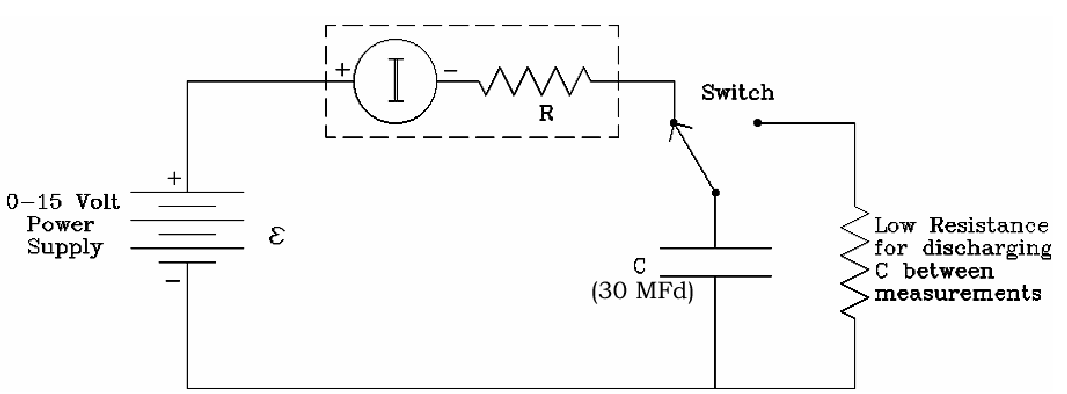
\includegraphics[width=0.8\textwidth]{./Exp4/pic/image6.png}
    \end{center}
    \caption{Large RC-charging Circuit}
    \label{fig:largerccharge}
\end{figure}

\begin{itemize}
  \item Measure $I$ at a series of time intervals after closing the switch. Plot $\ln,I$ vs. $t$ and construct a best-fit line.
  \item Use LINEST to determine the slope of your best-fit line with error.
  \item From your slope, determine the time constant $RC$ with error.
  \item Does your calculated time constant agree with the theoretical value $RC$ determined from the resistance and capacitance of the circuit?
\end{itemize}

\subsection{Large RC-discharging}

Use the circuit shown in Fig. \ref{fig:largercdischarge} to measure the discharge current through the resistance $R$ of the same capacitors $C$ used in Part 1. You will use the same equipment as you used in Part 1 of the lab. \myskip

\begin{figure}[h]
    \begin{center}
        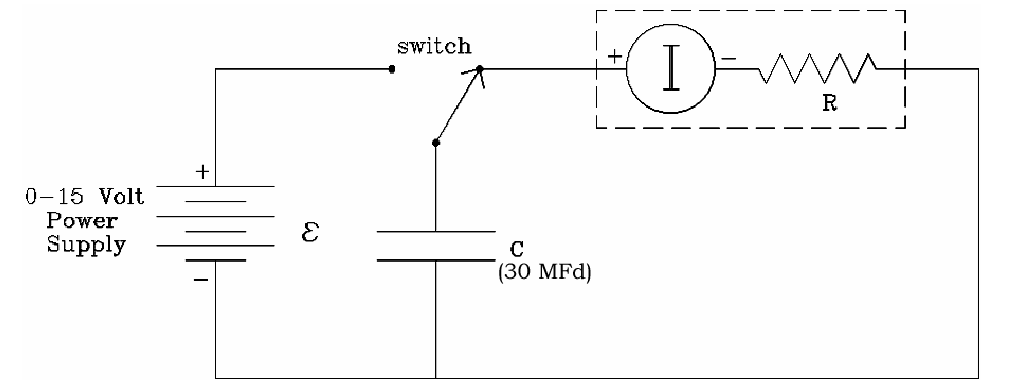
\includegraphics[width=0.65\textwidth]{./Exp4/pic/image7.png}
    \end{center}
    \caption{Large RC-discharging Circuit}
    \label{fig:largercdischarge}
\end{figure}

Before closing the switch to begin the measurement, momentarily connect the power supply directly across the capacitor in order to give it an initial charge.
\begin{itemize}
  \item Disconnect the power supply, close the switch, and measure $I$ as a function of time. Plot $\ln,I$ vs $t$ and construct a best fit line.
  \item Use LINEST to determine the slope of your best-fit line with error.
  \item From your slope, determine the time constant $RC$ with error.
  \item Does your calculated time constant agree with the theoretical value $RC$ determined from the resistance and capacitance of the circuit?
\end{itemize}

\subsection{A Relaxation Oscillator}

A neon bulb has the property of having a very high resistance (almost infinite) until the voltage applied to it is high enough to ``break down'' the gas, at which point the bulb lights and its resistance becomes very low. In this part of the lab you will use a high voltage power supply. Thus, \emph{it is essential that you are sure to use the small capacitor with a value of $0.082\,\mathrm{\mu F}$} rather than the bank of capacitors you use in the first two parts of the lab. Wire a neon bulb in parallel with the capacitor in the circuit of figure \ref{fig:relaxcirc}.\myskip

\begin{figure}[h]
    \begin{center}
        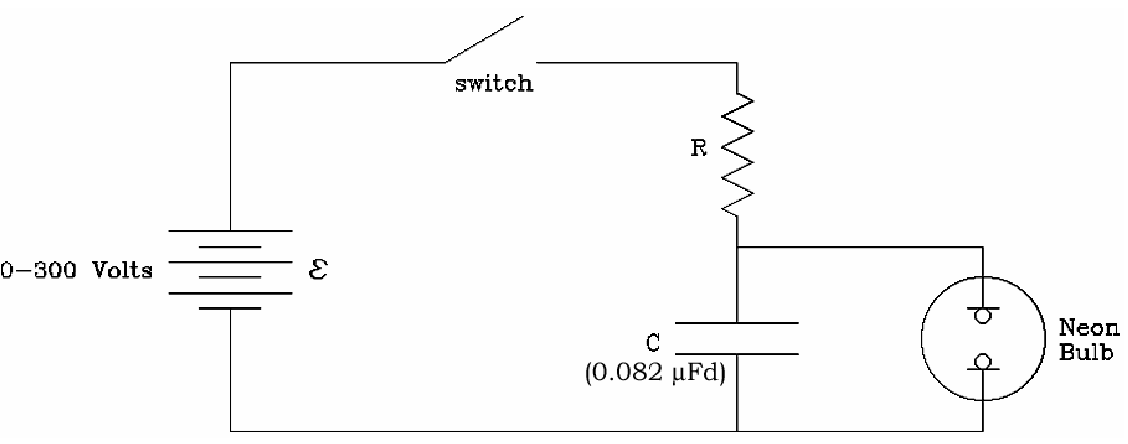
\includegraphics[width=0.75\textwidth]{./Exp4/pic/image8.png}
    \end{center}
    \caption{Relaxation Oscillator Circuit}
    \label{fig:relaxcirc}
\end{figure}

\textbf{CAUTION}: Since a relatively \underline{high-voltage} power supply is necessary for this part of the experiment, it is important not to touch any exposed metal parts of the circuit while the power supply is connected to the circuit and turned on, whether or not the switch is closed. Since the capacitor stores charge, \emph{it may be charged even if the voltage supply has been removed}. Be sure to discharge the capacitor fully by simultaneously touching an insulated wire to each end of the capacitor before touching any of the metal parts of the circuit.\myskip

When the switch is closed, the capacitor will start to be charged as in Part 1 with the time constant $RC$. The high resistance  of the neon bulb will have negligible effect on the circuit since it is wired in parallel. However, when the capacitor is charged to sufficiently high voltage, the neon bulb will light. The capacitor will then be quickly discharged through the bulb. If $R$ is sufficiently large, there will not be sufficient current to keep the bulb lit after the capacitor is discharged. The bulb will then be extinguished; it will return to a state of high resistance, and the charging process will start again. For a given applied voltage $\varepsilon$, and a neon bulb with a given breakdown voltage, the period of this repetitive ``oscillation'' will thus be determined by the value of $RC$.\myskip
\begin{itemize}
  \item Measure the period for different combinations of $R$ and $C$ (at least three combinations) with error. Error in period $\tao$ can be found from the precision of the measuring instrument.
  \item Verify the dependence of $\tao$ on the product of $RC$ by plotting $\tao$ vs. $RC$ in Excel. Make sure to include error bars and a line of best-fit.
  \item Determine the slope of your line with error using LINEST.
  \item How might you interpret the slope of your line?
  \item Discuss the major sources of error in measuring the period $\tao$ in this experiment.
\end{itemize}
